\documentclass[a4paper]{article}

%import packages
\usepackage[utf8]{inputenc}
\usepackage{graphicx}
\usepackage{wrapfig}
\usepackage{float}
\usepackage{listings}
\usepackage{amsmath}
\usepackage{epigraph}
\usepackage{multicol}
\usepackage[a4paper, total={7in, 8in}]{geometry}

%define variables
\newcommand{\projectname}{0xchan}

%set up header
\title{\projectname}
\author{
  sumpunk\\
  \texttt{sumpunk@protonmail.com}
  \and
  ARitz Cracker\\
  \texttt{aritz@aritzcracker.ca}
}

\begin{document}

\maketitle

\begin{figure}[H]
    \centering
    \texttt{WORKING DRAFT v1.0.6}

\end{figure}

\begin{abstract}
\projectname{} is a decentralized and immutable message board system on the Ethereum blockchain where users can post messages and media files. Storage of those messages is handled via IPFS and a smart contract is used to store a ledger of all messages. A Proof of Stake style mechanism ensures quality content and protects the system against spam, while also incentivising users to stake their Ether. The immutable and decentralized nature of the system allows for free speech and gives way to create truly censorship resistant and self sustaining platforms.

\end{abstract}

\section*{Acknowledgement}
This project is a collaborative effort between sumpunk (full stack) and ARitz Cracker (solidity). 

We thank ToCsIcK for cross-checking solidity codebase and ideas as well as helping out with full stack development.

We thank our community staff Capex, Crypto McPump, Cryptoknight, EthRabbi, kadaz, Lil Stronghands, Ms Incognito and SciPanda for keeping the Discord server in check and maojk for being the translating bridge to our chinese community.

We thank our voluntary community support and helpdesk staff for swiftly answering community questions.

We also thank Vitalik Buterin for creating Ethereum in the first place.

\vspace*{\fill}
\epigraph{I disapprove of what you say, but I will defend to the death your right to say it.}{Evelyn Beatrice Hall}

\pagebreak

\section{What \projectname{} is}
Like many other dApps \projectname{} consists of a website that interfaces with a smart contract. The contract serves as a decentralized ledger to write to and read from while larger chunks of data are stored on the decentralized IPFS network. The smart contract and the storage is decentralized, the website however is not. Users can clone or fork the website repository and set up another interface by themselves and either host it for others to use as well or run it on a local webserver for themselves.

\begin{figure}[H]
  \centering
  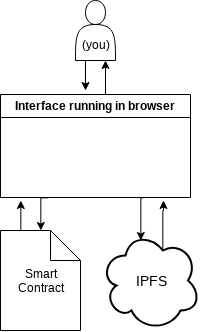
\includegraphics[width=0.25\textwidth]{0x_flow.png}
  \caption{Simplified interaction flow between users, smart contract and IPFS}
  \label{fig:flow}
\end{figure}

By crafting the necessary transaction data themselves, users could also send messages directly to the smart contract through the use of tools like MyEtherWallet or Etherscan or even command line interfaces. There is no way to restrict a user from sending messages to the contract.

The messages sent to the system usually consist of at least a short or long comment made by the user, an optional subject and optional media attachments. This allows users to freely express their thoughts, discuss various topics and engage with ongoing discussions or start new ones. All of this happens free from censorship by government or other authorities.

\section{What IPFS is}
IPFS, or the ``InterPlanetary FileSystem'' is a self described peer-to-peer hypermedia protocol to make the web faster, safer, and more open.

It relies on users operating so called nodes to distribute server load and content storage across multiple machines with a certain level of redundancy.

Nodes will keep stored content as long as the node has it pinned. If content gets unpinned it will be purged from the node once no more requests for that content are made to preserve storage space. Users can set up their own nodes and require them to replicate data from another node they specify. That way a network can be established with redundancy.

Users can interact with IPFS either through the use of a command line interface, desktop or mobile applications, or by using web interfaces.

More on IPFS can be read in their own whitepaper\footnote{IPFS Whitepaper https://github.com/ipfs/papers/raw/master/ipfs-cap2pfs/ipfs-p2p-file-system.pdf}.

\section{Decentralization and immutability}
As stated before, data on IPFS can \emph{vanish} if the content is unpinned and when not enough requests are made for the content to be saved from the IPFS garbage collector tool, although the deletion propagates very slowly as most files remain inside a node's cache for a prolonged period of time and can be retrieved by requesting the file again. 

By default, 0xchan.net will operate it's own IPFS node which other users can tap into and replicate to create redundant data storage. They can also choose to refuse garbage collection on their nodes which makes it possible to further keep files even though they are removed on the replicated node.

If content is deleted on a node and is being re-added to the same node directory, the generated hash will remain the same. This will always be the case if users use the 0xchan.net interface to upload their files, since it'll always use the same directories.

The immutability stems from the fact that the smart contract can never be stopped at any time unless the entire Ethereum network is halted. As more users deploy their own nodes to replicate the 0xchan.net node, the level of decentralization rises and by not allowing files to be arbitrarily deleted the content distribution network becomes immutable as well.

By hosting their own nodes and participating in the content distribution, users are also strengthening the network against single point of failures and censorship by the operator of the 0xchan.net node.

\section{Using \projectname}
Users can either browse \projectname{} and just read the conversations or actively participate in them. Simply browsing the dApp for content comes at no extra cost to the user, while posting a comment will invoke a fee. This prevents spam bots from using \projectname{} as a dumping ground for malicious or otherwise irritating content, so users can focus on real human to human discussions.

\subsection{Proof of Stake}
The requirement for each user that wants to post on \projectname{} is to have a minimum of 0.5 Ether locked in the contract. This will be used as stake and collateral at the same time. Staking requirement for sending messages with attachments is an additional 1.5 Ether. The Ether sent as stake can be withdrawn by the users anytime if they did not post in the past 24 hours and there are no pending reports.

The stake will also assign users a certain percentage in the distributed rewards system.

Stake can be deposited by either using the proper functions of the smart contract or by simply sending Ether to the contract's address. The default action for received Ether is to turn it into stake. If the maximum amount of 2 Ether that can be staked is reached, additional Ether will be used to purchase ZCH.

\subsubsection{ZCH}
Each post sent to \projectname{} costs an additional 0.0001 Ether fee which is distributed among all stake holders (80\%) will purchase P3D (15\%) and a portion of it will stay in the contract to be used to settle expenses (5\%).

This fee should make it expensive enough for people to not spam the system with useless content, but low enough to allow for easy entry into free discussions. The price for a message can and should be adjusted to meet market conditions.

Users can also pay this fee in advance by purchasing ZCH, an ERC-20 token. This will also increase their overall percentage in the stake sharing pool. When users choose to use ZCH to pay for a post, they will only have to pay the Ethereum network fee which is kept at the lowest minimum possible due to gas optimization processes in the smart contract.

There is only a theoretical limit to the amount of ZCH that can ever be minted but the contract does not have a restriction on the maximum supply for ZCH. The use of ZCH burns the token.

\subsubsection{\projectname{} and P3D}
\projectname{} will put the 15\% of the posting fee into a pool which will purchase P3D tokens\footnote{PoWH3D Wiki (2018) https://powh3d.hostedwiki.co/} from the P3D smart contract. The pool will be managed by the \projectname{} smart contract and users can force a purchase whenever they like, however it won't be possible to use a masternode\footnote{A so called ``masternode'' is a referral program used by P3D} during those purchases. This will generate dividends for the P3D network but the contract will also receive those dividends just the same. The dividends collected that way will be released to all ZCH token holders everytime a new P3D purchase is made.

\subsection{Posting a message}
Users will make use of the website's input forms similar to the one in figure \ref{fig:input} to create their threads and replies, as well as attach media files to their posts.

\begin{figure}[H]
  \centering
  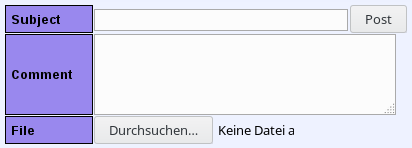
\includegraphics[width=0.6\textwidth]{0x_4chan_post.png}
  \caption{Example for an input field as found on 4chan}
  \label{fig:input}
\end{figure}

Since storing data on the Ethereum blockchain is quite expensive in terms of gas cost, we push the comment data and optional images to IPFS and only write a modified storage hash to our smart contract ledger. Since IPFS returns a hash that starts with ``Qm'' in it's base configuration, we can strip the first two bytes of the returned hash and use cheaper storager for a ``byte32'' entity since the modified hash will be exactly 32 bytes long. We can safely assume that other node operators will not change the default hashing behavior and thus reconstruct the hash on the interface.

\begin{figure}[H]
  \centering
  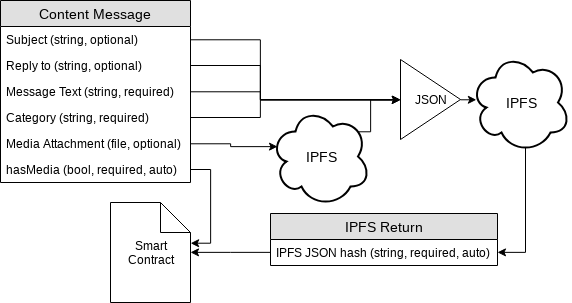
\includegraphics[width=0.6\textwidth]{0x_logic.png}
  \caption{Disassembly of a message to 0xchan and storage procedure, content stored is subject to change}
  \label{fig:logic}
\end{figure}

All text based key values will be transformed into a single JSON object, images will be added as they are to the IPFS node. The frontend will initiate the process, wait until the files have been added and pinned and return their IPFS hashes accordingly so the transaction can be properly written to the blockchain.

\subsubsection{Temporary content}
To increase user experience \projectname{} is going to make use of the user's browser localstorage, which allows safe and temporary storing of data similar to how cookies work. When a user creates a new post or thread, the data will not only be sent to IPFS but also stored in the localstorage and \projectname{} will use that to display the content that was sent to IPFS to the user.

Since localstorage is a local unit, other users will not see the content. This will be made clear in a little notification attached to the message. Once the user submitted transaction on the Ethereum network has been processed, other users will also be able to see the content and interact with it. 

The user's localstorage for temporary content will be purged regularly either automatically or it can be purged manually by the user.

\subsubsection{Interacting with posts}
Each post can be interacted with in many ways, replying to them is just one of those possibilities.

Users can award each other \emph{(you)} tokens that can be collected and later be redeemed for cosmetic things. (you) don't account for any additional stake nor can they be traded or sold.

Another way to thank users for a post would be through an integrated \emph{donation} function that engages a standard Ether transfer from the user clicking the button on 0xchan.net to the user that made the post where users can choose how much Ether will be sent themselves. No Ether will be transferred to the \projectname{} contract that way. Feature inclusion do be decided for final release of whitepaper.

\subsubsection{Dropping of posts}
Each board can hold a maximum amount of pages ($A\textsubscript{p}$) worth of threads. Each new thread pushes all other threads back in the hierarchy of ordering when first created. Order changes with each reply to each individual thread. If a new thread would put the total amount of threads to $A\textsubscript{p}+1$, the ``oldest'' thread in the storage array would be dropped from the smart contract's index. Nodes can query this index to understand if they can unpin content and free up storage for new content.

\subsection{User profiles}
Each user will have an automatically populated profile page displaying their address, amount of posts made, amount of ZCH and stake, amount of (you) awarded and some other things that may get added with future extensions. Since the profile page will be populated using the currently used Ethereum address, the page may only be viewed by the owner of the profile.

The page also serves as a hub to manage ZCH balances, withdrawal of outstanding rewards, stake deposit and withdrawal.

\subsection{Creation of custom boards}
Users will have the opportunity to create their own so called \emph{boards}. Boards serve as a general filter for categories of various interests, i.e. automobiles, photography, drawing but also adult themed content like pornography, fetishes and so on.

To create a board users can either send a creation transaction directly by calling the corresponding function from Etherscan or similar tools, or by using a form on the website. The creation process of a board will ask the user for a shortcode for the board that should not be larger than 4 letters or numbers (i.e. \emph{wsg}), a complete name (i.e. \emph{Work Safe GIF}) and a short description of the content the creator would like to see on that board (i.e. \emph{A collection of safe for work animated images}).

The creation process will burn 100 ZCH from the user's account or if the user doesn't have 100 ZCH to burn ask for 0.01 Ether which will be distributed in the same way as a regular posting fee.

\projectname{} will provide a few default boards at launch to serve as a base, custom boards can be added post launch. The list of available boards will be automatically updated each time a new board has been added.

\subsubsection{Removal of custom boards}
To remove cruft and keep the smart contract performant, the removal of custom boards is a necessary step. Users can not remove the boards themselves, instead the contract has to be queried from within the interface to check for unused boards.

A board becomes unused if there has been no new post or thread in a timeframe of 1 month. After that period the board will be open to removal.

The process is fairly simple. Users can manually query the contract through the interface and will be presented with a list of boards that are deemed ``unused''. They can then initiate a transaction which removes the boards from storage.

\subsection{Moderation}
\begin{wrapfigure}{r}[32pt]{0.5\textwidth}
    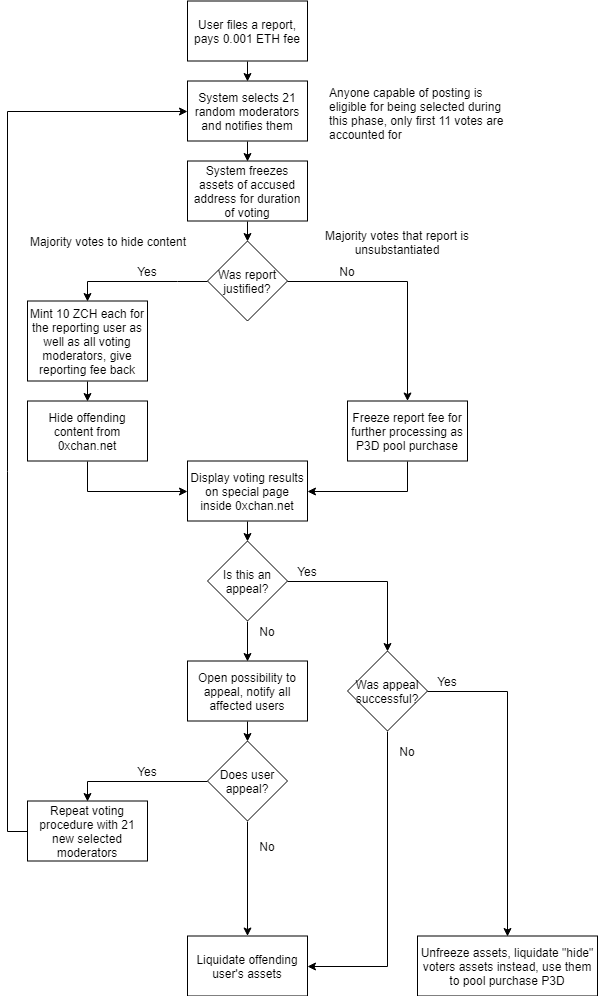
\includegraphics[width=0.4\textwidth]{0x_moderation.png}
    \caption{Simplified flow of reporting process, moderation voting and appeal process}
    \label{fig:mod}
\end{wrapfigure}

Since \projectname{} aims to give the power of moderation to its actual userbase instead of enabling despotism, no elaborate additional scheme like \emph{Delegated Proof of Stake} will take place, as those are regularly prone to abuse by accounts with enough funding and will subsequently turn a free speech and unregulated platform into a place of collusion and voting fraud.

The moderation process starts with a report from a user, which costs 0.001 Ether and will set in motion following mechanics:

\begin{enumerate}
    \item Freezing of the accused user's Stake (Ether)
    \item Suspension of transfer of user's ZCH to addresses other than the contract
    \item Letting the moderation contract select 21 randomly chosen accounts to vote on this issue
\end{enumerate}

Selection of voters will take place inside a smart contract to increase the level of transparency for the users. The first 11 votes will be accounted for, all other votes will be rejected. If the majority votes for a permanent hiding of the offending content, \emph{all participating voters and the reporting user} are granted 10 ZCH each, the reporting user will receive their reporting fee back and the content will be hidden permanently on 0xchan.net; if the majority thinks the report was false, the reporting fee will be frozen and depending on the outcome of a possible appeal will be used to purchase P3D. The option to vote on a report will stay open for 7 days.

Voting results will be displayed on a page hosted with 0xchan.net and users can file for appeals from within that page. Should they choose to appeal, 21 new users will be selected to vote and essentially repeat the previous process once more. Appealing does not incur additional fees. The option to appeal stays available for 7 days. Should the user choose not to appeal will the liquidation of their assets take place; the ZCH will be burned and the staked Ether will be used to purchase P3D.

If an appeal was successful, the accused user's assets will be unfrozen, the hidden content will be visible again and the assets of the voters who initially voted to permanently hide the content will be liquidated instead; ZCH will be burned and the staked Ether will be used to purchase P3D.

A report will be discarded if less than 11 votes are cast on it, or if the maximum time to live for the report is reached (7 days in this example). The reporting fee will be scheduled to be refunded to the reporter and no action will take place regarding the content.

The moderation contract is a seperately deployed contract which can be dynamically linked to the \projectname{} main contract. This allows us to update the codebase should any issues arise or new features be needed.

\subsection{Withdrawal or reinvesting of user funds}
Since users are subject to receiving a reward based on their staked amount and total amount of ZCH in posession, the website will also provide an easy to use withdrawal functionality where users can always see how much Ether has accumulated since the last withdrawal and then decide to move that to their wallet, or use the funds to directly purchase ZCH instead.

\section{Using your ZCH for other things}
ZCH are the main currency for \projectname{} and can be used for more than just pre-purchasing posting permissions.

\subsection{Purchasing wordfilters DRAFT}
A wordfilter is an automatic process which takes the original word and replaces it with a target word, chosen by the user buying the rights to deploy the wordfilter. On 4chan for example wordfilters exist to change for example the abbreviated phrase ``tbh'' into ``desu'', following the ``desu-meme'' of around 2006\footnote{"Desu on Know Your Meme", https://knowyourmeme.com/memes/desu}.

Users can purchase the right to enact their own wordfilters to all other users\footnote{Please note that this feature will only be visible on 0xchan.net and other access points hosting the same frontend codebase.} by using the supplied interface. By making use of a slightly modified version of a Harberger Tax based system\footnote{"What is Harberger Tax \& Where Does The Blockchain Fit In?", Simon de la Rouviere (July 2018) https://medium.com/@simondlr/what-is-harberger-tax-where-does-the-blockchain-fit-in-1329046922c6} the users can enjoy this feature as a kind of mini-game on top of \projectname{}.

The price ($P$) of the wordfilter is determined by the user purchasing it, however they will have to stake 50\% of the sales price as a liquidity pool ($L$), which the system uses to deduct a 2\% daily tax ($P\textsubscript{t}$). The system will automatically remove the wordfilter again should the funding of the current owner run out. A new wordfilter can be bought to replace the currently registered filter by paying $P$ Following example should make it easier to understand how the procedure of acquiring a wordfilter, funding it and replacing an existing wordfilter works.

Assume User A determines the wordfilter is worth $P=100$ ZCH. Taking the previous rules into account User A would have to deposit $L$ amount of ZCH (in this case a total of 50 ZCH) to keep the liquidity pool funded. The system will deduct the daily tax in a manner of $P\textsubscript{t}=\frac{P}{100} \times 2$. If User B decides to buy the wordfilter, User A would receive the price of the filter $P$ as well as a refund ($R$) of the tax in a manner of $R=P\textsubscript{t} \times T$ where $T$ is defined by taking into account the run time of the wordfilter in days, multiplied by the tax amount per day. User B can now also determine a new Price $P$ for the wordfilter (ideally at a higher price than what User B paid) and has to pay $P\textsubscript{t}$ on the newly defined $P$ just as User A had to do before.

There can only be one active word filter at any given time per board. Users wanting to create new wordfilters will have to either be the first to activate them, or purchase the rights to existing wordfilters should a wordfilter already exist.

\section{Crowdfunding participants}
Users who participated in the crowdfunding campaign will be able to trade their ZCI tokens in a ratio of 1:1 with the smart contract and receive ZCH in return. This will be done by using a function on the \projectname{} smart contract which takes ZCI as payment and returns that payment with the ZCH token.

\pagebreak
\section*{Changelog}
\begin{itemize}
\item Oct. 02, 2019 (v1.0.6): Changelog permanently moved to Git, added section 4.2.1 
\item Oct. 01, 2019 (v1.0.5): Added sections 4.2.2 and 4.4.1
\item Sep. 29, 2019 (v1.0.4): Changed draft section 5.1 from banners to wordfilters
\item Sep. 11, 2019 (v1.0.3): Removed mention of Team JUST from first page
\item Mar. 2, 2019 (v1.0.2): Added draft section of system to enable users to purchase site banners employing Harberger Tax, mainly inspired by Troopy
\item Jan. 10, 2019 (v1.0.1): Added Changelog; changed functionality of moderation process to not freeze ZCH of accused user, but instead only prohibit transfer to other addresses to still allow for posting
\item Jan. 2, 2019 (v1.0.0): Release of Working Draft
\end{itemize}

\end{document}
